% TeXLocal test document: a book in several files.
%
% What to try with it:
%  - The sidebar's file tree: folders two deep, a file name with a space,
%    images, a bibliography, a Markdown note and a CSV file.
%  - Opening each kind of file: TeX in the editor, images and PDFs as previews.
%  - SyncTeX from the PDF into the chapter files, and from them to the PDF.
%  - The bibliography: biblatex through BibTeX, which latexmk runs as needed.
%    Change backend=bibtex to backend=biber to see a tool fail: this Mac's
%    TeX Live biber can't unpack itself ("extracting arm64 binary with lipo
%    failed"), and the citations stay undefined.
%  - Renaming, moving and deleting files in the sidebar, and adding files in
%    Finder while the project is open.
\documentclass[11pt]{report}
\usepackage[T1]{fontenc}
\usepackage{graphicx}
\usepackage{booktabs}
\usepackage{lipsum}
\usepackage[backend=bibtex, style=authoryear]{biblatex}
\usepackage{hyperref}
\addbibresource{references.bib}
\graphicspath{{figures/}}

% \includeonly{chapters/results}

\title{A Test Book for TeXLocal}
\author{The TeXLocal Test Documents}

\begin{document}

\maketitle
\tableofcontents
\listoffigures

\chapter{Introduction}\label{ch:intro}

This book is split across files. This chapter is \texttt{chapters/introduction.tex};
Chapter~\ref{ch:methods} is in \texttt{chapters/methods.tex}, and the appendix is
a folder deeper, in \texttt{chapters/appendix/derivations.tex}.

Citations come from \texttt{references.bib}: \textcite{knuth1984} wrote the
program, \textcite{lamport1994} the macros, and \textcite{mittelbach2023} the
companion \parencite[see also][]{oetiker2023}.

\section{Background}
\lipsum[1-3]

\section{Outline of the Book}
\lipsum[4-5]

\chapter{Methods}\label{ch:methods}

\section{Materials}
\lipsum[6-7]

Figure~\ref{fig:photo} is a PNG and Figure~\ref{fig:diagram} a PDF, both in
the \texttt{figures} folder.

\begin{figure}[ht]
  \centering
  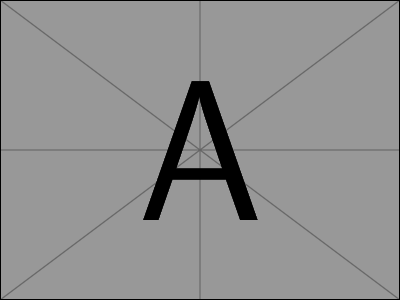
\includegraphics[width=0.6\linewidth]{photo}
  \caption{A PNG image (\texttt{figures/photo.png}).}\label{fig:photo}
\end{figure}

\section{Procedure}
\lipsum[8-10]

\begin{figure}[ht]
  \centering
  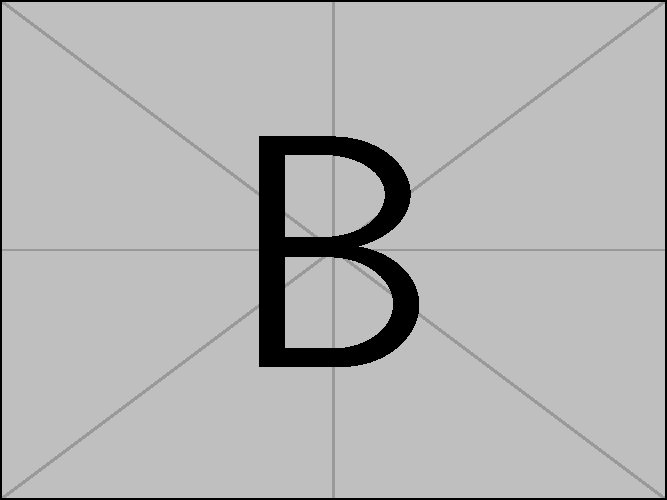
\includegraphics[width=0.6\linewidth]{diagram}
  \caption{A PDF image (\texttt{figures/diagram.pdf}).}\label{fig:diagram}
\end{figure}

\chapter{Results}\label{ch:results}

The numbers in Table~\ref{tab:data} are also in \texttt{data/results.csv}.

\begin{table}[ht]
  \centering
  \caption{Results by trial.}\label{tab:data}
  \begin{tabular}{crr}
    \toprule
    Trial & Time (s) & Error \\
    \midrule
    1 & 12.4 & 0.031 \\
    2 & 11.9 & 0.027 \\
    3 & 12.1 & 0.029 \\
    \bottomrule
  \end{tabular}
\end{table}

\section{A Wide Figure}
Its file name has a space in it: \texttt{figures/wide figure.pdf}.

\begin{figure}[ht]
  \centering
  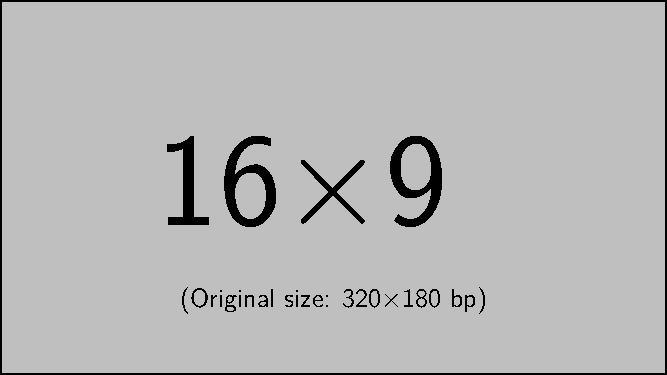
\includegraphics[width=\linewidth]{wide figure}
  \caption{A 16:9 image whose file name has a space.}\label{fig:wide}
\end{figure}

\section{Discussion}
\lipsum[11-14]


\chapter{Related Work}
% This file's name has a space in it, and it's \input, not \include.

\section{Typesetting Systems}
\TeX{} \parencite{knuth1984} and \LaTeX{} \parencite{lamport1994} are the
subject of this chapter. \lipsum[15]

\section{Editors}
\lipsum[16-17]


\appendix
\chapter{Derivations}
% Two folders deep: chapters/appendix/derivations.tex.

\section{The First Derivation}
Starting from
\begin{equation}
  y' = ky, \qquad y(0) = y_0,
\end{equation}
separating variables gives $\ln y = kt + C$, so $y = y_0 e^{kt}$.

\section{The Second Derivation}
\lipsum[18]


\printbibliography[heading=bibintoc]

\end{document}
